\section{Results}
\label{Results}
To test the code we have used a image almost similar to the one used in \parencite{Baoming2016}, the only difference is the size of the image. We have chosen to use a image with a lower resolution, because the program was running wary slow, when the image was larger then 300 x 300 pixels. \\
On \autoref{fig:original} the grey scale image used in this mini project can be seen.On \autoref{fig:r225} the resulting images from Equation 5 in \autoref{Step1} can be seen. On \autoref{fig:T} the resulting image of the differential equations in \autoref{Step3} , before the thresholding have been done. Hereafter the images is only noise which mostly looks like a QR code. This is a result of one or more errors in the code, which we haven't been able to detect.
\begin{figure}[H]
	\centering
	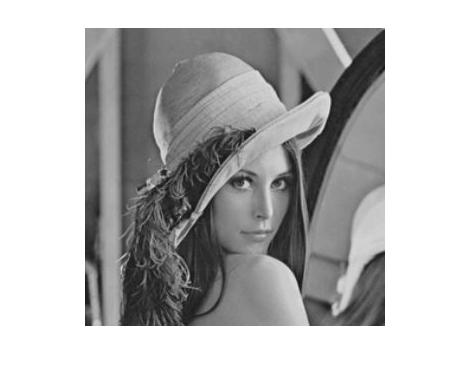
\includegraphics[resolution=300,scale=1.5]{/I}
	\caption{}
	\label{fig:original}
\end{figure}
\noindent
\begin{figure}[H]
	\centering
	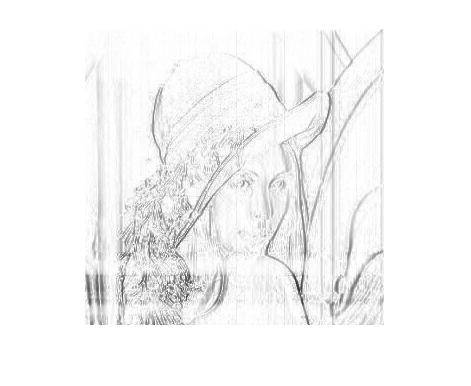
\includegraphics[resolution=300,scale=1.5]{/r255}
	\caption{}
	\label{fig:r225}
\end{figure}
\noindent
\begin{figure}[H]
	\centering
	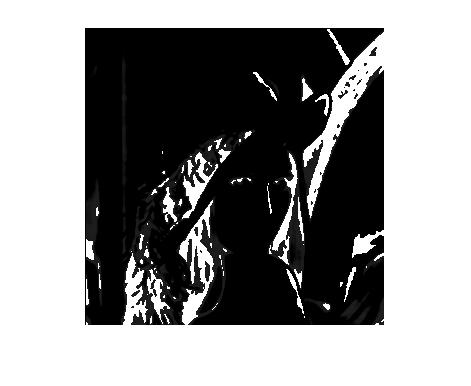
\includegraphics[resolution=300,scale=1.5]{/T}
	\caption{}
	\label{fig:T}
\end{figure}
\noindent
